% =====================================================================
%  EPD-SDIA-4112 -- Statistique Bayesienne -- Master 1 SDIA
%  CHAPITRE 2 : Distributions a priori et a posteriori   (50 slides, 8 h)
%  Fichier A : section 2.1 -- conjugaison
% =====================================================================
\section{Chapitre 2 --- A priori et a posteriori}
\chapterslide{Chapitre 2}{Distributions a priori et a posteriori}{8 h --- 5 sections --- 50 slides}{%
\textbf{Objectifs} --- écrire la loi a posteriori sous forme close grâce à la
conjugaison ; choisir un a priori en mesurant son information (uniforme, faiblement
informatif, Jeffreys, référence) ; valider ce choix par un contrôle prédictif a priori ;
quantifier la robustesse du posterior et le \emph{shrinkage} d'un modèle hiérarchique.}

% ---------------------------------------------------------------- 1
% [suite]
\begin{frame}{Objectifs pédagogiques du chapitre 2}
\begin{columns}[t]
\begin{column}{0.48\textwidth}
\begin{kbox}[Savoirs]
\begin{itemize}
  \item Écrire la loi a posteriori en forme close et reconnaître un noyau conjugué
  \item Distinguer les quatre couples conjugués classiques et leur mise à jour
  \item Classer les a priori : non informatif, faiblement informatif, informatif,
        Jeffreys, référence, propre ou impropre
  \item Expliquer la vitesse $1/\sqrt{n}$ de dominance des données
  \item Définir le \emph{shrinkage} et le pooling partiel d'un prior hiérarchique
\end{itemize}
\end{kbox}
\end{column}
\begin{column}{0.48\textwidth}
\begin{abox}[Savoir-faire évalués]
\begin{itemize}
  \item Dériver le posterior Beta-Binomial à la main, en trois lignes
  \item Faire tourner un contrôle prédictif a priori en PyMC avant toute donnée
  \item Calibrer l'échelle d'un prior pour exclure les valeurs impossibles
  \item Détecter la subtilité du prior uniforme sur un paramètre d'échelle
  \item Justifier un power prior devant un auditoire critique
\end{itemize}
\end{abox}
\end{column}
\end{columns}
\vspace{2mm}
\end{frame}

% [suite]
\begin{frame}{Objectifs pédagogiques du chapitre 2 (suite)}
\begin{tcolorbox}[colback=byLight,colframe=byGrey!50,arc=2mm,width=.95\textwidth]
\centering\small
\textbf{Évaluation} — TP noté PyMC (10 \%) \;|\; quiz de fin de section (5 \%) \;|\;
examen final écrit (85 \%). \textbf{Prérequis} : chapitre 1 (théorème de Bayes, loi prédictive).
\end{tcolorbox}
\end{frame}

% ---------------------------------------------------------------- 2
% [suite]
\begin{frame}{Plan du chapitre 2 (8 h)}
% [rogna]
\small
\begin{enumerate}
  \item[2.1] \textbf{Conjugaison et couples conjugués} \hfill \textit{frames 2--18}
  \item[2.2] \textbf{Choisir un a priori} \hfill \textit{frames 19--27}
  \item[2.3] \textbf{Contrôles prédictifs a priori} \hfill \textit{frames 28--35}
  \item[2.4] \textbf{Robustesse, sensibilité, \emph{shrinkage}} \hfill \textit{frames 36--45}
  \item[2.5] \textbf{Synthèse et bonnes pratiques} \hfill \textit{frames 46--51}
\end{enumerate}
\vspace{2mm}
\begin{center}
\begin{tabular}{@{}p{1.2cm}p{5.6cm}p{3.0cm}p{2.4cm}@{}}
\toprule
\textbf{Section} & \textbf{Question directrice} & \textbf{Outil principal} & \textbf{Livrable} \\
\midrule
2.1 & Peut-on éviter les intégrales ? & Couples conjugués & Tableau de conjugaison \\
2.2 & Quel a priori est défendable ? & Jeffreys, élicitation & Fiche de prior \\
2.3 & Ce prior prédit-il l'impossible ? & \py{pm.sample_prior_predictive} & Graphique de contrôle \\
2.4 & Combien de données pour l'effacer ? & Power prior, hiérarchie & Courbe de sensibilité \\
2.5 & Que retenir pour le projet ? & Recommandations & Checklist \\
\bottomrule
\end{tabular}
\end{center}
\end{frame}

% [suite]
\begin{frame}{Plan du chapitre 2 (8 h) (suite)}
\begin{tcolorbox}[colback=byPurple!6,colframe=byPurple,arc=2mm,width=.95\textwidth]
\small\centering
\textbf{Fil rouge} — un posterior n'est jamais donné : il est \emph{construit} par un choix
(a priori) et \emph{évalué} par comparaison avec ce qu'on sait du phénomène.
\end{tcolorbox}
\end{frame}

% ---------------------------------------------------------------- 3
\begin{frame}{La recette en trois gestes}
\begin{ebox}[Méthode : multiplier, puis reconnaître]
\begin{enumerate}
  \item \textbf{Écrire le prior} : $p(\theta) \propto \prod_j \theta_j^{\,a_j - 1}$
        (noyau d'une loi connue).
  \item \textbf{Écrire la vraisemblance} : $p(y \given \theta) \propto
        \prod_j \theta_j^{\,s_j}$ pour les modèles i.i.d. exponentiels.
  \item \textbf{Multiplier et identifier} : les exposants s'\textbf{additionnent},
        $a_j \mapsto a_j + s_j$ : on reconnaît le noyau du posterior.
\end{enumerate}
\[
p(\theta \given y) \;\propto\; \underbrace{p(\theta)}_{\text{exposants } a_j - 1}
\;\times\; \underbrace{p(y \given \theta)}_{\text{exposants } s_j}
\;=\; \prod_j \theta_j^{\,a_j + s_j - 1}
\]
\end{ebox}
\vspace{1mm}
\begin{columns}[t]
\begin{column}{0.57\textwidth}
\begin{kbox}[La question utile sur la constante]
Le posterior est connu \textbf{à une constante près} :
$p(y) = \int p(y \given \theta) p(\theta)\,\mathrm{d}\theta$, une intégrale sans
forme close. La conjugaison retrouve cette constante par
\textbf{identification d'un noyau connu} : on ne calcule jamais l'intégrale.
\end{kbox}
\end{column}
\begin{column}{0.39\textwidth}
\begin{ebox}[Vérification numérique]
Avec le noyau identifié $\mathrm{Beta}(8, 17)$, la densité est exacte :
$\int_0^1 \theta^{7}(1-\theta)^{16}\mathrm{d}\theta = B(8,17)$,
constante que SciPy évalue en $1{,}70 \cdot 10^{-7}$ sans aucune quadrature
adaptative.
\end{ebox}
\end{column}
\end{columns}
\end{frame}

% ---------------------------------------------------------------- 4
\begin{frame}{Pourquoi la conjugaison simplifie (et ce qu'elle coûte)}
% [rogna]
\footnotesize
\begin{columns}[t]
\begin{column}{0.50\textwidth}
\begin{ebox}[Le même posterior, trois coûts]
Pour le modèle Beta-Binomial de Challenger ($n = 23$, $k = 7$) :
\begin{itemize}
  \item \textbf{Conjugué} : $\mathrm{Beta}(1+7,\,1+23-7) = \mathrm{Beta}(8,17)$,
        exact, temps machine négligeable ;
  \item \textbf{Grille} : $10^6$ points, précision limitée, coût $n^{d}$ en dimension $d$ ;
  \item \textbf{MCMC (NUTS, 2 chaînes de 2000 tirages)} : posterior retrouvé,
        mais $41{,}2$~s de calcul et un diagnostic à vérifier ($\hat R = 1{,}0016$).
\end{itemize}
\vspace{1mm}
\centering\small Les trois chemins donnent la même loi : seul le \emph{contrat} change
(exactitude contre généralité).
\end{ebox}
\end{column}
\begin{column}{0.47\textwidth}
\begin{kbox}[Quatre bénéfices réels]
\begin{itemize}
  \item \textbf{Exactitude} : aucune approximation, aucun critère de convergence ;
  \item \textbf{Vitesse} : mise à jour en $O(1)$, embarquable (spam, flotte de capteurs) ;
  \item \textbf{Interprétation} : le prior $a+b$ se lit comme un \emph{échantillon virtuel} ;
  \item \textbf{Pédagogie} : c'est le banc d'essai qui permet de \emph{vérifier} un
        échantillonneur MCMC (chapitre 5).
\end{itemize}
\end{kbox}
\begin{wbox}[Ce qu'elle coûte]
La classe conjuguée est \textbf{étroite} : dès qu'on empile des paramètres
(hiérarchie, mélanges, valeurs manquantes), on retombe sur le calcul numérique.
La conjugaison est un raisonnement, pas une religion.
\end{wbox}
\end{column}
\end{columns}
\end{frame}

% ---------------------------------------------------------------- 5
\begin{frame}{Tableau récapitulatif des conjugaisons}
\centering
\renewcommand{\arraystretch}{1.25}
\begin{tabular}{@{}p{3.3cm}p{3.2cm}p{2.9cm}p{3.3cm}@{}}
\toprule
\textbf{Vraisemblance} & \textbf{A priori conjugué} & \textbf{A posteriori} &
\textbf{Mise à jour} \\
\midrule
$\mathrm{Bin}(n,\theta)$ & $\mathrm{Beta}(a,b)$ &
$\mathrm{Beta}(a+k,\,b+n-k)$ & succès $\to a$, échecs $\to b$ \\[1mm]
$\mathrm{Poisson}(\lambda)$ & $\mathrm{Gamma}(\alpha,\beta)$ &
$\mathrm{Gamma}(\alpha + \sum y_i,\;\beta + n)$ & comptes $\to \alpha$,
expositions $\to \beta$ \\[1mm]
$\N(\mu, \sigma^2)$ avec $\sigma$ connu & $\N(\mu_0, \tau^2)$ &
$\N\!\big(\mu_n, \tau_n^2\big)$ & précisions qui s'additionnent \\[1mm]
$\mathrm{Multinomiale}(n, p)$ & $\mathrm{Dirichlet}(\alpha)$ &
$\mathrm{Dirichlet}(\alpha + x)$ & comptes par catégorie $\to \alpha_j$ \\[1mm]
$\mathrm{Exp}(\lambda)$ & $\mathrm{Gamma}(\alpha, \beta)$ &
$\mathrm{Gamma}(\alpha + n,\;\beta + \sum y_i)$ & mêmes règles que Poisson \\[1mm]
\bottomrule
\end{tabular}
\vspace{2mm}
\begin{itemize}
  \item[$\blacktriangleright$] \textbf{Recette normalisée} (Normal-Normal) :
        $\dfrac{1}{\tau_n^2} = \dfrac{1}{\tau^2} + \dfrac{n}{\sigma^2}$ \quad et \quad
        $\mu_n = \tau_n^2\!\left(\dfrac{\mu_0}{\tau^2} + \dfrac{n \bar y}{\sigma^2}\right)$.
  \item[$\blacktriangleright$] \textbf{Forme unique} : posterior $\propto$ prior $\times$
        vraisemblance ; les hyperparamètres perdent le nom de « paramètres de loi »
        et deviennent des \emph{compteurs de données virtuelles}.
\end{itemize}
\end{frame}

% ---------------------------------------------------------------- 6
\begin{frame}{Les familles de priors et leurs moments}
\begin{center}
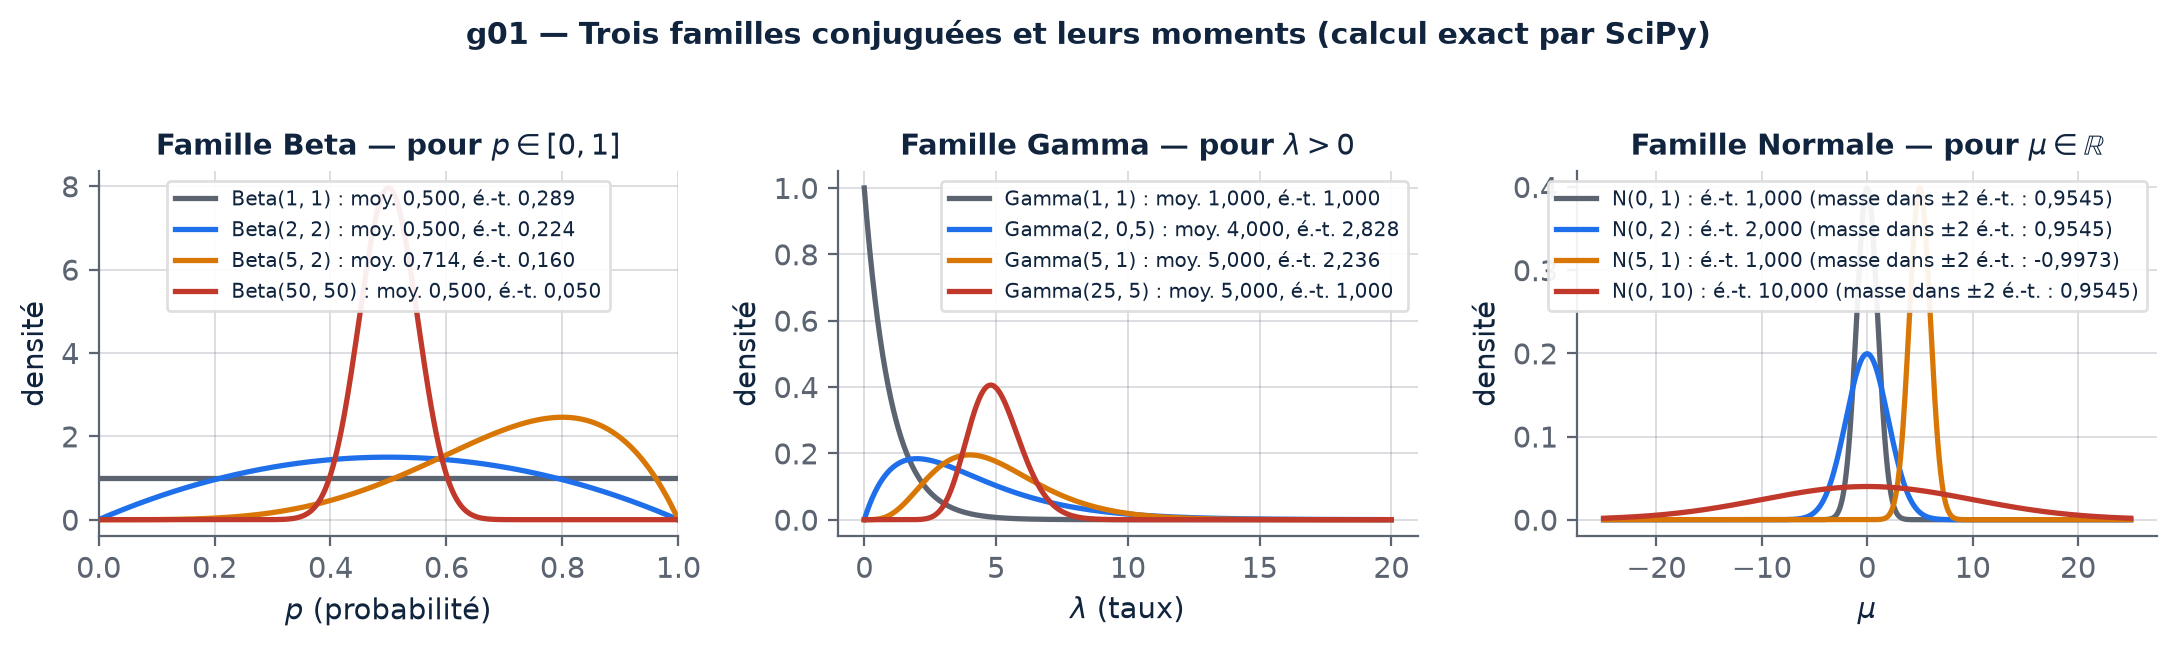
\includegraphics[width=0.74\textwidth]{g01_familles_priors.png}
\end{center}
\vspace{-1mm}
\begin{columns}[t]
\begin{column}{0.55\textwidth}
\begin{kbox}[Lire les hyperparamètres]
\begin{itemize}
  \item $\mathrm{Beta}(a,b)$ : moyenne $\frac{a}{a+b}$, écart-type
        $\sqrt{\frac{ab}{(a+b)^2(a+b+1)}}$ ; $a+b$ est la \emph{taille} de l'échantillon virtuel.
  \item $\mathrm{Gamma}(\alpha,\beta)$ : moyenne $\alpha/\beta$, écart-type
        $\sqrt{\alpha}/\beta$ ; attention au paramétrage \emph{rate} contre \emph{scale}.
  \item $\N(\mu_0,\tau^2)$ : la précision $1/\tau^2$ est l'information apportée.
\end{itemize}
\end{kbox}
\end{column}
\begin{column}{0.42\textwidth}
\begin{ebox}[Valeurs calculées (SciPy)]
$\mathrm{Beta}(1,1)$ : é.-t. $0{,}2887$ \;|\; $\mathrm{Beta}(2,2)$ : $0{,}2236$ \;|\;
$\mathrm{Beta}(50,50)$ : $0{,}0498$.\\
$\mathrm{Gamma}(1,1)$ : é.-t. $1{,}000$ \;|\; $\mathrm{Gamma}(25,5)$ : $0{,}200$\\
$= \sqrt{\alpha}/\beta = 5/5$ : resserrer un prior ne change pas sa moyenne.
\end{ebox}
\end{column}
\end{columns}
\end{frame}

% ---------------------------------------------------------------- 7
% [split]
\begin{frame}{Beta-Binomial : le cas d'école de Challenger}
\begin{center}
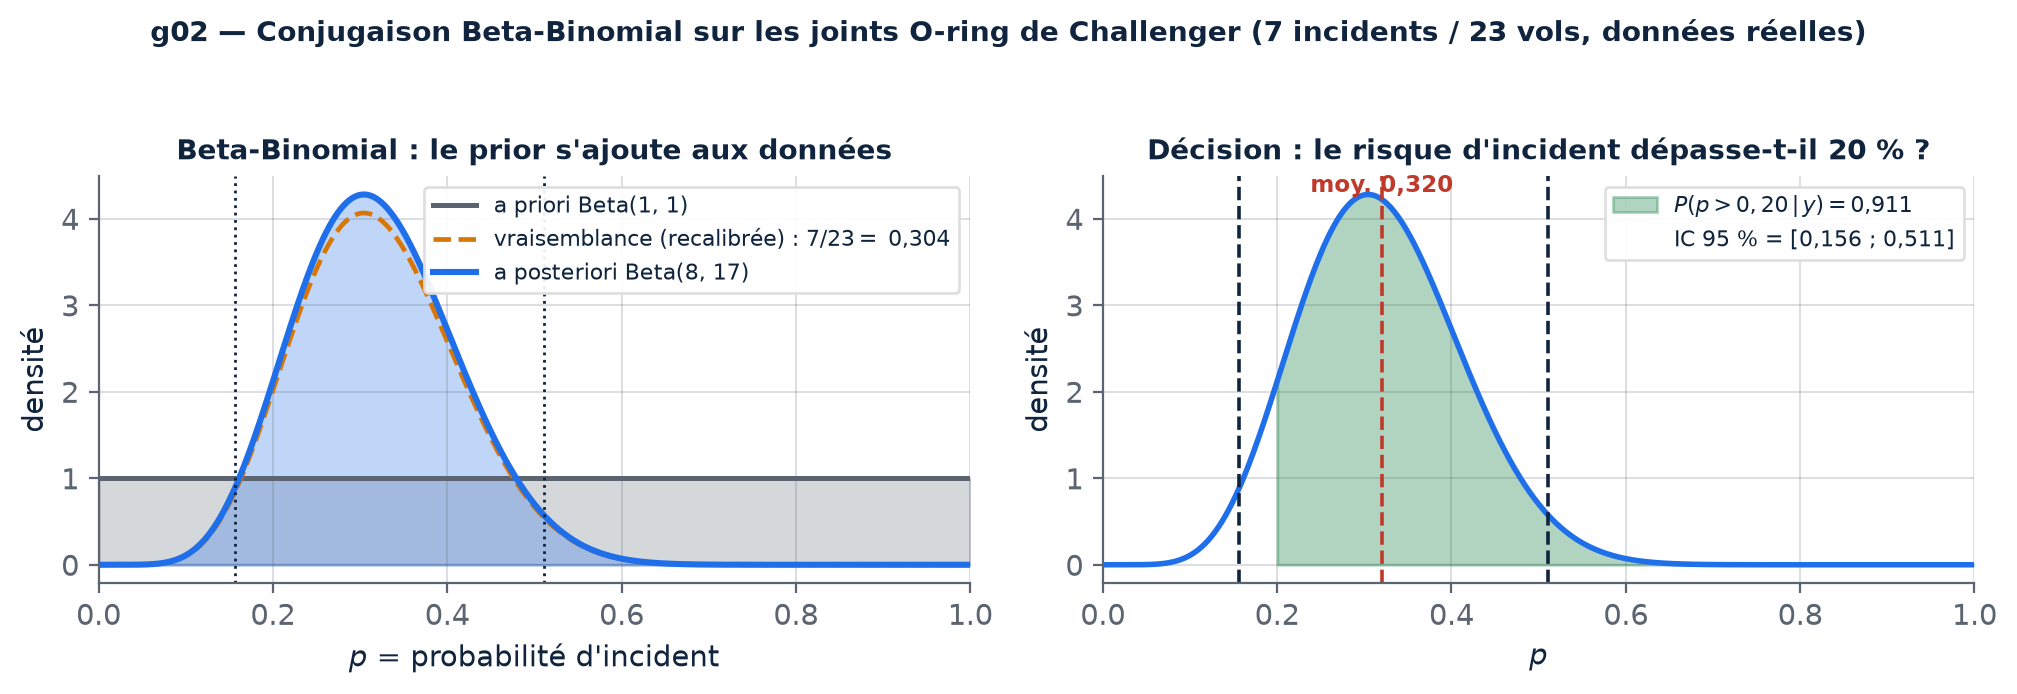
\includegraphics[width=\textwidth]{g02_conjugue_beta_binomial.png}
\end{center}
\end{frame}

% [split]
% [suite]
\begin{frame}{Beta-Binomial : le cas d'école de Challenger}
% [rogna]
\small
\begin{columns}[t]
\begin{column}{0.45\textwidth}
\begin{ebox}[Données réelles (Challenger)]
23 vols de la navette avant la catastrophe : \textbf{7 vols} présentent une
dégradation thermique des joints O-ring. Modèle :
\[
p \sim \mathrm{Beta}(1,1), \qquad k \given p \sim \mathrm{Bin}(23, p)
\]
Posterior conjugué : $\mathrm{Beta}(1+7,\,1+23-7) = \mathbf{Beta(8,17)}$.
\end{ebox}
\begin{solbox}[Résultats exécutés]
\begin{itemize}
  \item Moyenne a posteriori $\mathbf{0{,}320}$, écart-type $0{,}0915$
  \item IC 95 \% : $[0{,}156 \,;\, 0{,}511]$
  \item $P(p > 0{,}20 \given y) = \mathbf{0{,}911}$ : la question décisionnelle
  \item $P(p > 0{,}50 \given y) = 0{,}032$
\end{itemize}
\end{solbox}
\end{column}
\end{columns}
\vspace{1mm}
\end{frame}

% [suite]
\begin{frame}{Beta-Binomial : le cas d'école de Challenger (suite)}
\begin{wbox}[Le prior d'ingénieur change la conclusion]
Avec l'avis d'expert « un joint qui casse dans 1 vol sur 40 » encodé en
$\mathrm{Beta}(1{,}3,\,50)$ : posterior Beta$(8{,}3,\,66)$, moyenne
\textbf{0,112} et IC 95 \% $[0{,}051 \,;\, 0{,}192]$. Même données,
conclusion d'un facteur 3 près : \textbf{le prior doit être écrit et défendu}.
\end{wbox}
\end{frame}

% ---------------------------------------------------------------- 8
% [split]
\begin{frame}{Gamma-Poisson : le comptage de particules alpha (1910)}
\begin{center}
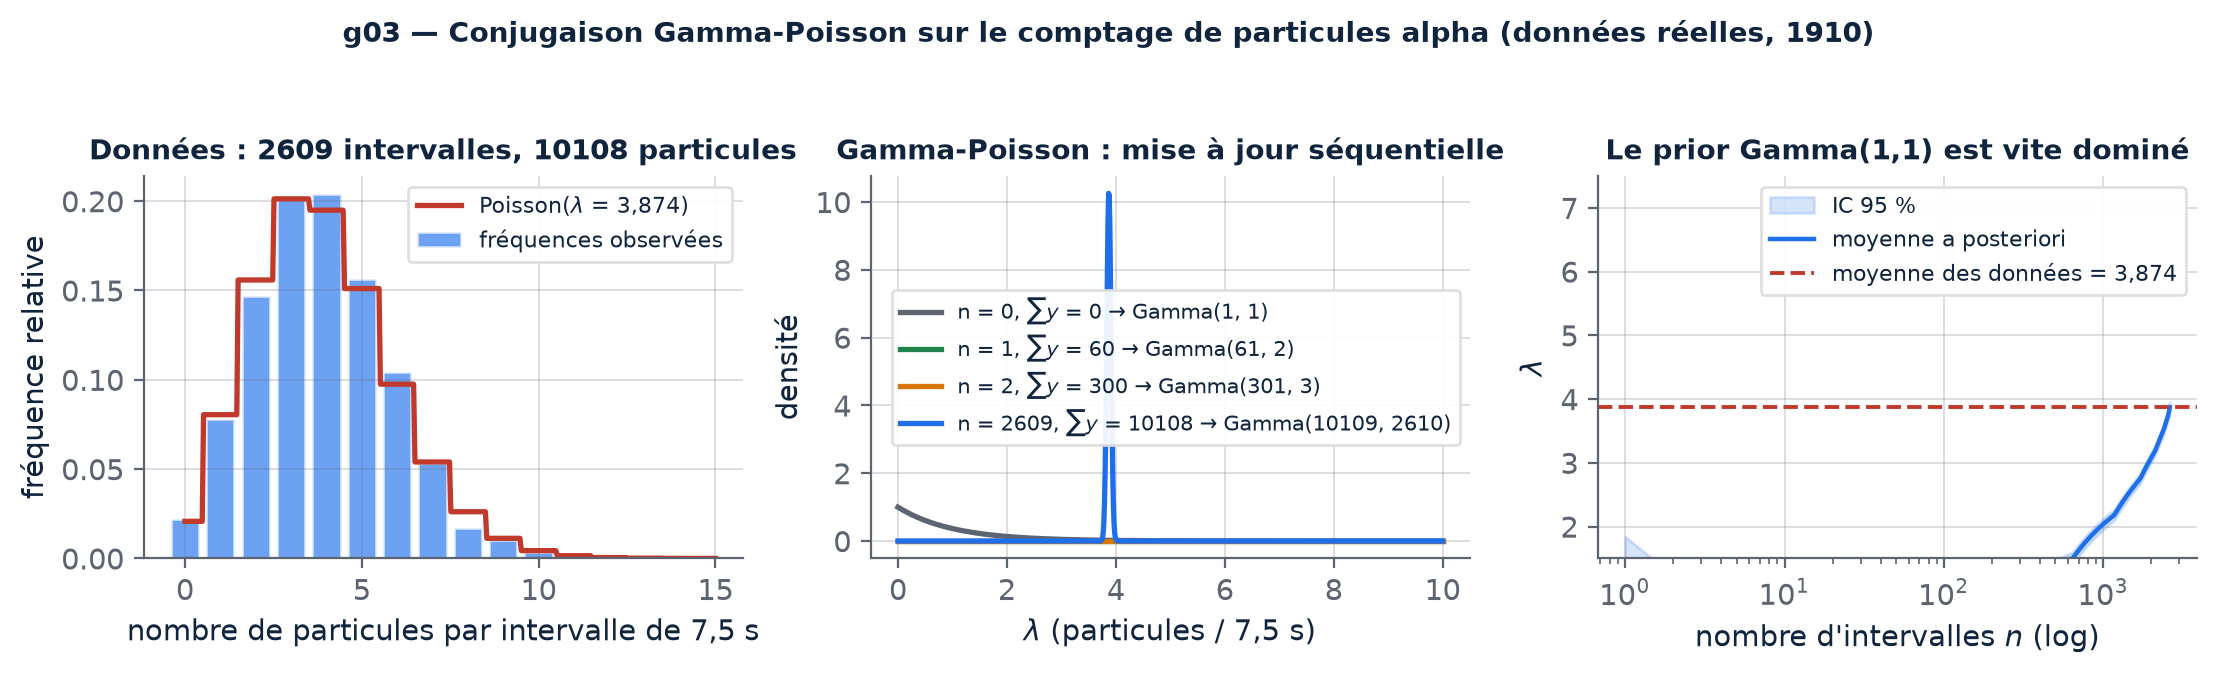
\includegraphics[width=\textwidth]{g03_conjugue_gamma_poisson.png}
\end{center}
\end{frame}

% [split]
% [suite]
% [suite5]
\begin{frame}{Gamma-Poisson : le comptage de particules alpha (1910)}
\begin{columns}[t]
\begin{column}{0.44\textwidth}
\begin{ebox}[Données réelles (Rutherford \& Geiger)]
Un compteur Geiger observe des particules alpha pendant des intervalles de 7,5 s.
Table de fréquences exploitée par le script :
\begin{itemize}
  \item $2\,609$ intervalles observés
  \item $10\,108$ particules comptées au total
  \item moyenne empirique $\bar y = \mathbf{3{,}8743}$
\end{itemize}
Modèle : $y_i \given \lambda \sim \mathrm{Poisson}(\lambda)$, prior $\mathrm{Gamma}(1,1)$.
\end{ebox}
\end{column}
\end{columns}
\vspace{1mm}
\end{frame}

% [suite5]
\begin{frame}{Gamma-Poisson : le comptage de particules alpha (1910) (suite)}
\begin{solbox}[Posterior conjugué]
\[
\mathrm{Gamma}\!\Big(1 + \sum_i y_i,\; 1 + n\Big)
= \mathrm{Gamma}(10\,109,\; 2\,610)
\]
moyenne $\mathbf{3{,}8732}$, écart-type $0{,}0385$, IC 95 \%
$[3{,}798 \,;\, 3{,}949]$.
\end{solbox}
\end{frame}

% [suite]
\begin{frame}{Gamma-Poisson : le comptage de particules alpha (1910) (suite)}
\begin{kbox}[Ce que la figure du milieu montre]
À droite, le prior ne pèse que $\frac{1}{1+n}$ : dès $n \approx 10$ intervalles
il est effacé. C'est la situation typique de la \textbf{détection de fraude} ou du
\textbf{comptage de défauts} : beaucoup d'observations, prior peu influent,
mise à jour séquentielle naturelle (on peut streamer : chaque nouveau compte
ajoute simplement 1 à $\alpha$ et 1 à $\beta$).
\end{kbox}
\end{frame}

% ---------------------------------------------------------------- 9
% [split]
\begin{frame}{Normal-Normal : une école, un bruit, un prior défendable}
\begin{center}
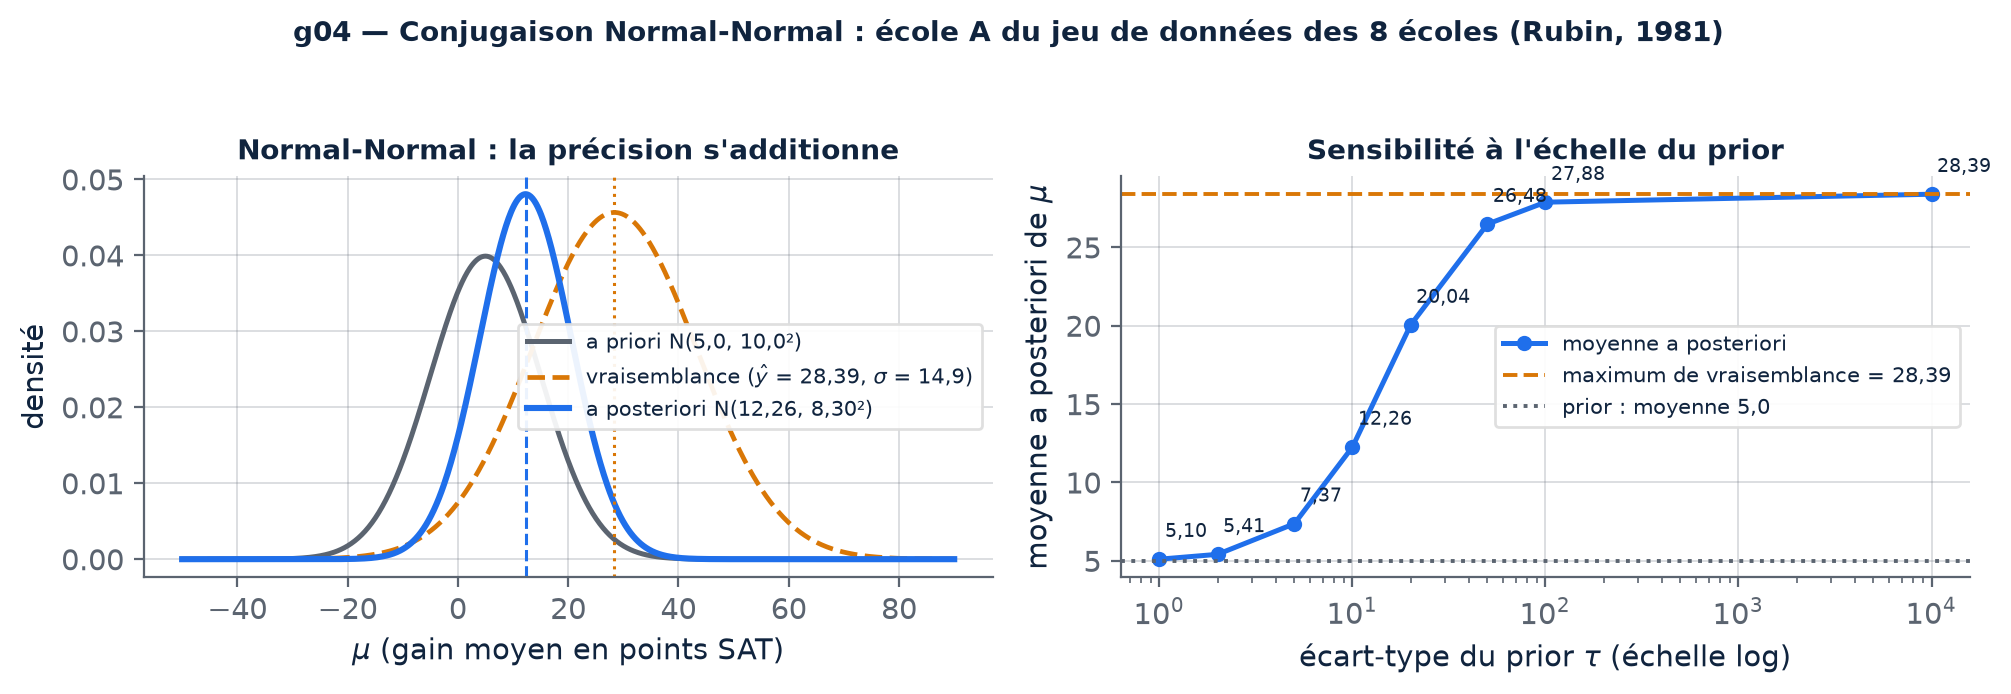
\includegraphics[width=\textwidth]{g04_conjugue_normal_normal.png}
\end{center}
\end{frame}

% [split]
% [suite5]
\begin{frame}{Normal-Normal : une école, un bruit, un prior défendable}
% [rogna]
\small
\begin{columns}[t]
\begin{column}{0.45\textwidth}
\begin{ebox}[Données réelles (Rubin, 1981)]
Le programme de préparation au SAT de l'école A est estimé à
$\hat y = 28{,}39$ points avec une erreur standard connue $\sigma = 14{,}9$.
Prior \emph{faiblement informatif} : $\mu \sim \N(5, 10^2)$.
\end{ebox}
\begin{solbox}[Posterior exact]
$\mu \given y \sim \N(12{,}2642,\; 8{,}3033^2)$, IC 95 \%
$[-4{,}01 \,;\, 28{,}54]$.\\[1mm]
Le posterior \textbf{contracte} l'estimation d'un facteur
$\mathbf{0{,}432}$ vers le prior.
\end{solbox}
\end{column}
\end{columns}
\end{frame}

% [suite5]
\begin{frame}{Normal-Normal : une école, un bruit, un prior défendable (suite)}
\begin{kbox}[Le levier est $\tau$, pas $\mu_0$]
$\tau = 1 \to 5{,}105$ ; $\tau = 5 \to 7{,}367$ ;
$\tau = 10 \to 12{,}264$ ; $\tau = 50 \to 26{,}482$ ; $\tau = 10^4 \to 28{,}390$
(le maximum de vraisemblance). Choisir $\tau$ \emph{calibre l'information}
apportée par l'expert.
\end{kbox}
\end{frame}

% ---------------------------------------------------------------- 10
% [split]
\begin{frame}{Dirichlet-Multinomial : les 556 pois de Mendel}
\begin{center}
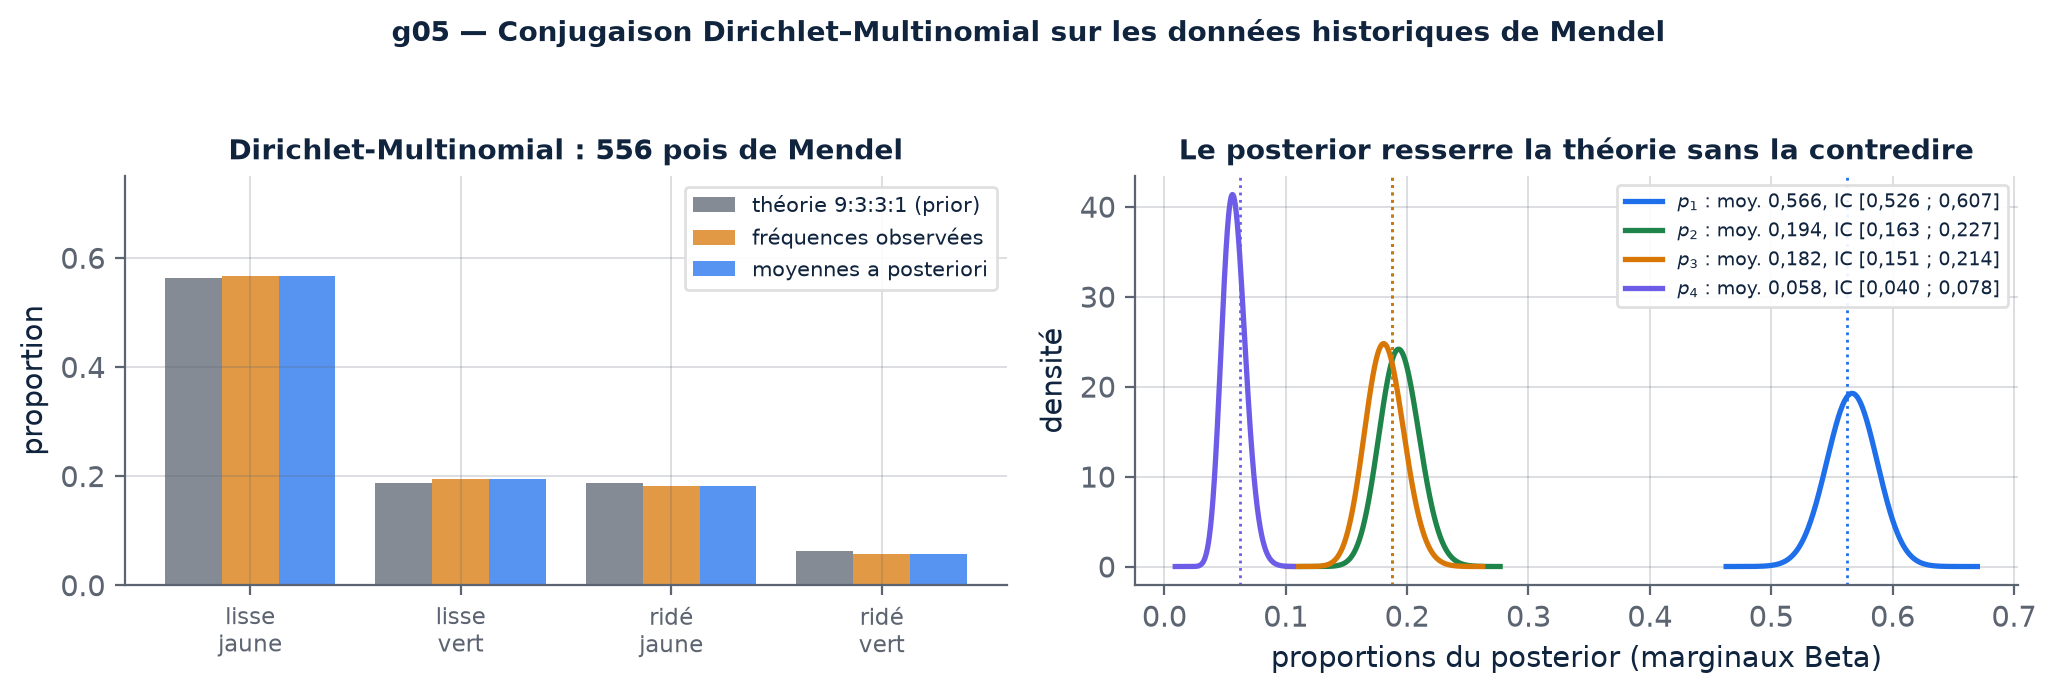
\includegraphics[width=\textwidth]{g05_conjugue_dirichlet_multinomial.png}
\end{center}
\end{frame}

% [split]
% [suite5]
\begin{frame}{Dirichlet-Multinomial : les 556 pois de Mendel}
% [rogna]
\small
\begin{columns}[t]
\begin{column}{0.45\textwidth}
\begin{ebox}[Données (Mendel, 1865)]
556 pois répartis en quatre phénotypes : lisse-jaune \textbf{315}, lisse-vert
\textbf{108}, ridé-jaune \textbf{101}, ridé-vert \textbf{32}. La théorie de Mendel
donne les proportions $9{:}3{:}3{:}1 = (0{,}5625 ; 0{,}1875 ; 0{,}1875 ; 0{,}0625)$.
\end{ebox}
\begin{solbox}[La théorie entre comme a priori]
$\alpha_0 = (9, 3, 3, 1)$ \;$\to$\;
$\mathrm{Dirichlet}(9+315,\,3+108,\,3+101,\,1+32) = \mathbf{Dirichlet(324, 111, 104, 33)}$
\end{solbox}
\end{column}
\end{columns}
\vspace{1mm}
\centering\small
\textbf{Lecture} — trois intervalles sur quatre contiennent la prédiction théorique :
le posterior \emph{resserre} la théorie sans la contredire. C'est exactement l'usage
d'une loi a priori comme \emph{hypothèse de travail falsifiable}.
\end{frame}

% [suite5]
\begin{frame}{Dirichlet-Multinomial : les 556 pois de Mendel (suite)}
\begin{kbox}[Les quatre marginaux]
$p_1$ : $0{,}5664$ \;$[0{,}5257;0{,}6068]$ (théorie $0{,}5625$) \;/\;
$p_2$ : $0{,}1941$ \;$[0{,}1627;0{,}2274]$ ($0{,}1875$) \\
$p_3$ : $0{,}1818$ \;$[0{,}1513;0{,}2144]$ \;/\;
$p_4$ : $0{,}0577$ \;$[0{,}0401;0{,}0782]$
\end{kbox}
\end{frame}

% ---------------------------------------------------------------- 11
% [rogna]
% [rogna]
% [rogna]
% [split]
\begin{frame}{Vue d'ensemble : quatre couples, un même mécanisme}
\begin{center}
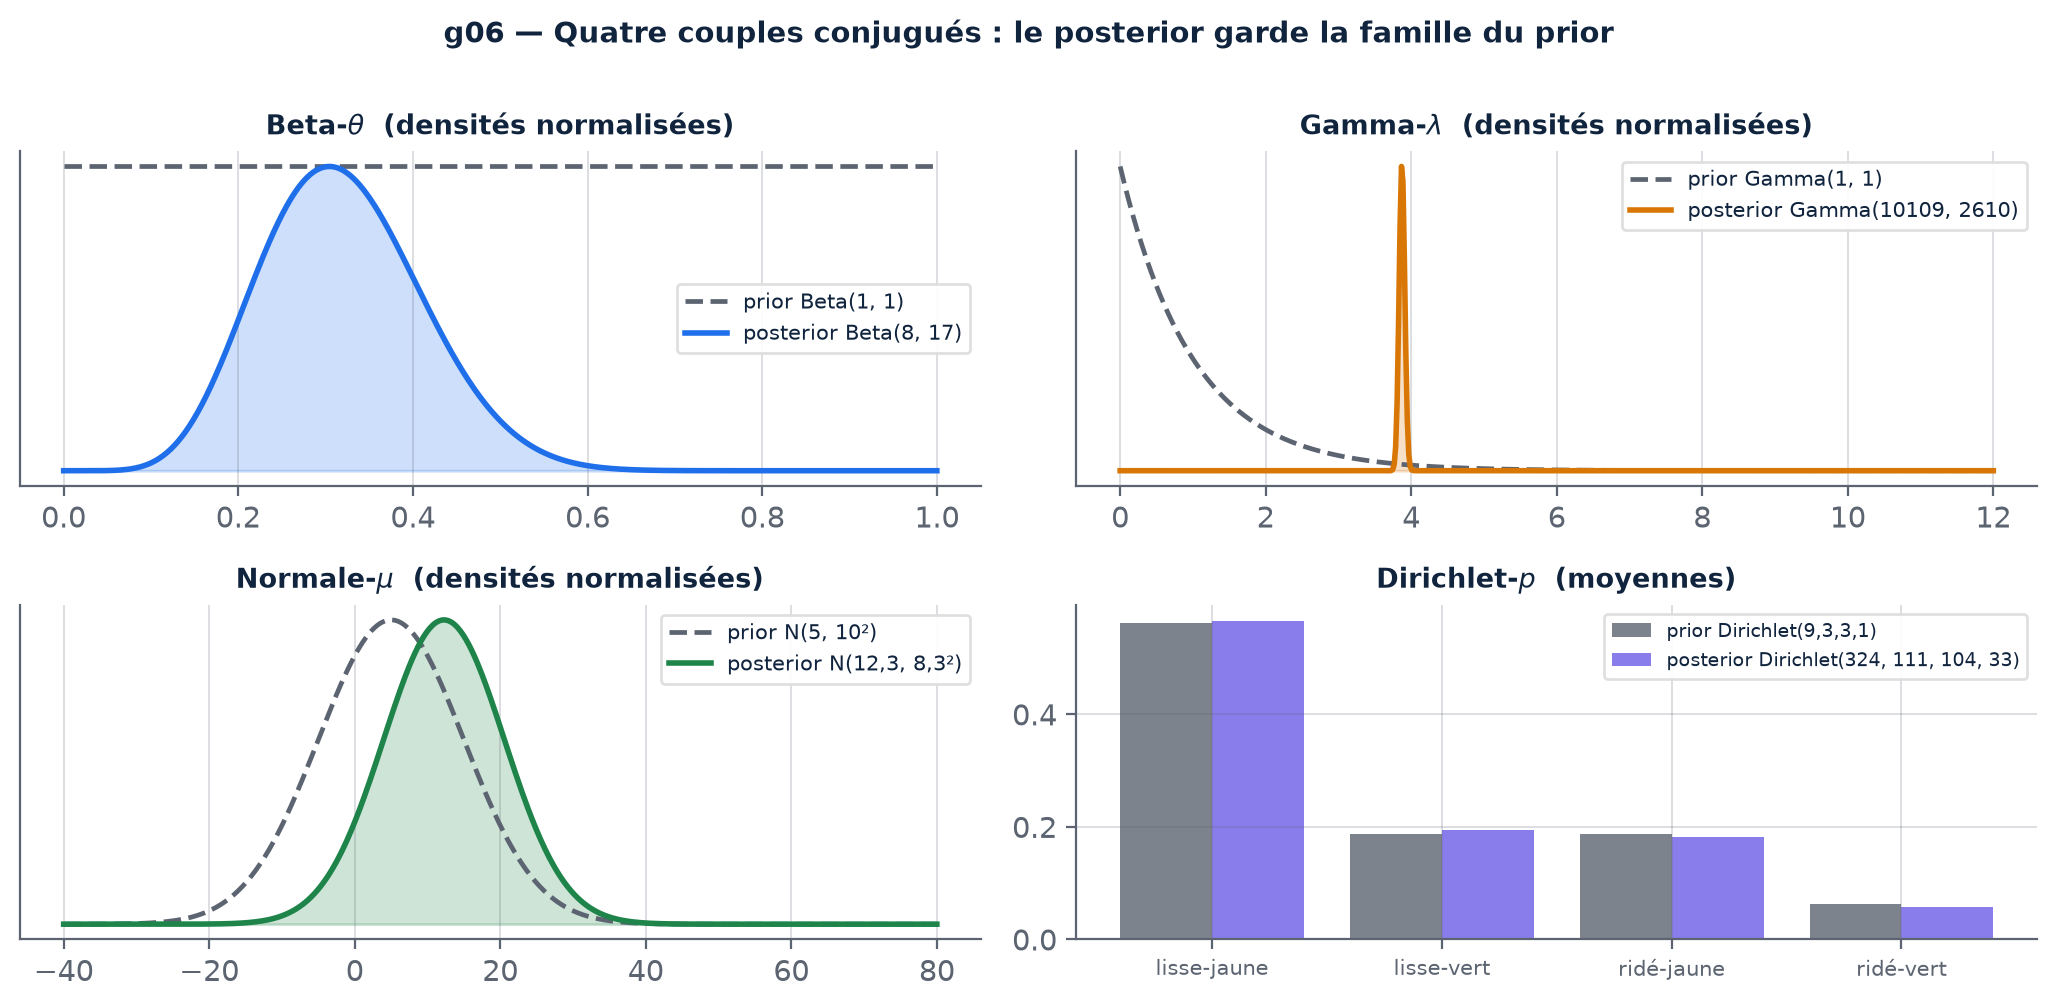
\includegraphics[width=.86\textwidth]{g06_quatre_trios.png}
\end{center}
\end{frame}

% [split]
\begin{frame}{Vue d'ensemble : quatre couples, un même mécanisme}

\vspace{-4mm}
\begin{columns}[t]
\begin{column}{0.48\textwidth}
\begin{kbox}[Ce que la figure prouve]
Dans les quatre cas, le posterior appartient à la \textbf{même famille} que le
prior : Beta $\to$ Beta, Gamma $\to$ Gamma, Normale $\to$ Normale,
Dirichlet $\to$ Dirichlet. Seuls les \emph{hyperparamètres} ont changé, et
toujours d'une seule manière : on a ajouté les données.
\end{kbox}
\end{column}
\begin{column}{0.48\textwidth}
\begin{ebox}[Le test à refaire en examen]
Écrire un modèle (vraisemblance + prior), dériver le noyau du posterior,
identifier la famille et ses paramètres, puis donner moyenne, mode et
intervalle de crédibilité. Quatre modèles au programme, cinq minutes chacun.
\end{ebox}
\end{column}
\end{columns}
\end{frame}

% ---------------------------------------------------------------- 12
\begin{frame}[fragile]{Vérification : le même posterior par PyMC (10 lignes)}
\begin{columns}[t]
\begin{column}{0.53\textwidth}
\begin{codebox}[src/fig\_ch2b\_pymc.py — modèle Beta-Binomial]
\begin{lstlisting}
import pymc as pm, arviz as az
import numpy as np

n_vols, k_incidents = 23, 7      # donnees reelles

with pm.Model() as m:
    p = pm.Beta("p", alpha=1, beta=1)   # prior uniforme
    pm.Binomial("y", n=n_vols, p=p,
                observed=k_incidents)

    idata = pm.sample(draws=2000, tune=1000,
                      chains=2, cores=1,
                      random_seed=42)

echantillons = idata.posterior["p"].values.ravel()
print(echantillons.mean())
print(np.percentile(echantillons, [2.5, 97.5]))
\end{lstlisting}
\end{codebox}
\end{column}
\begin{column}{0.44\textwidth}
\begin{kbox}[Le contrat de l'échantillonneur]
Aucune conjugaison, aucune dérivée à la main : on \emph{décrit} le modèle et
NUTS explore le posterior. Le prix est le diagnostic : $\hat R$, taille
d'échantillon efficace, autocorrélation.
\end{kbox}
\begin{solbox}[Résultat exécuté sur CPU]
Moyenne $0{,}3196$ \;;\; IC 95 \% $[0{,}1536 \,;\, 0{,}5138]$ \;;\;
$\hat R = 1{,}0016$ \;;\; ESS $\approx 1\,719$ \;;\; $41{,}2$~s.
\end{solbox}
\end{column}
\end{columns}
\end{frame}

% ---------------------------------------------------------------- 13
% [rogna]
% [rogna]
% [rogna]
\begin{frame}{Analytique contre échantillonnage : le match nul attendu}
\begin{center}
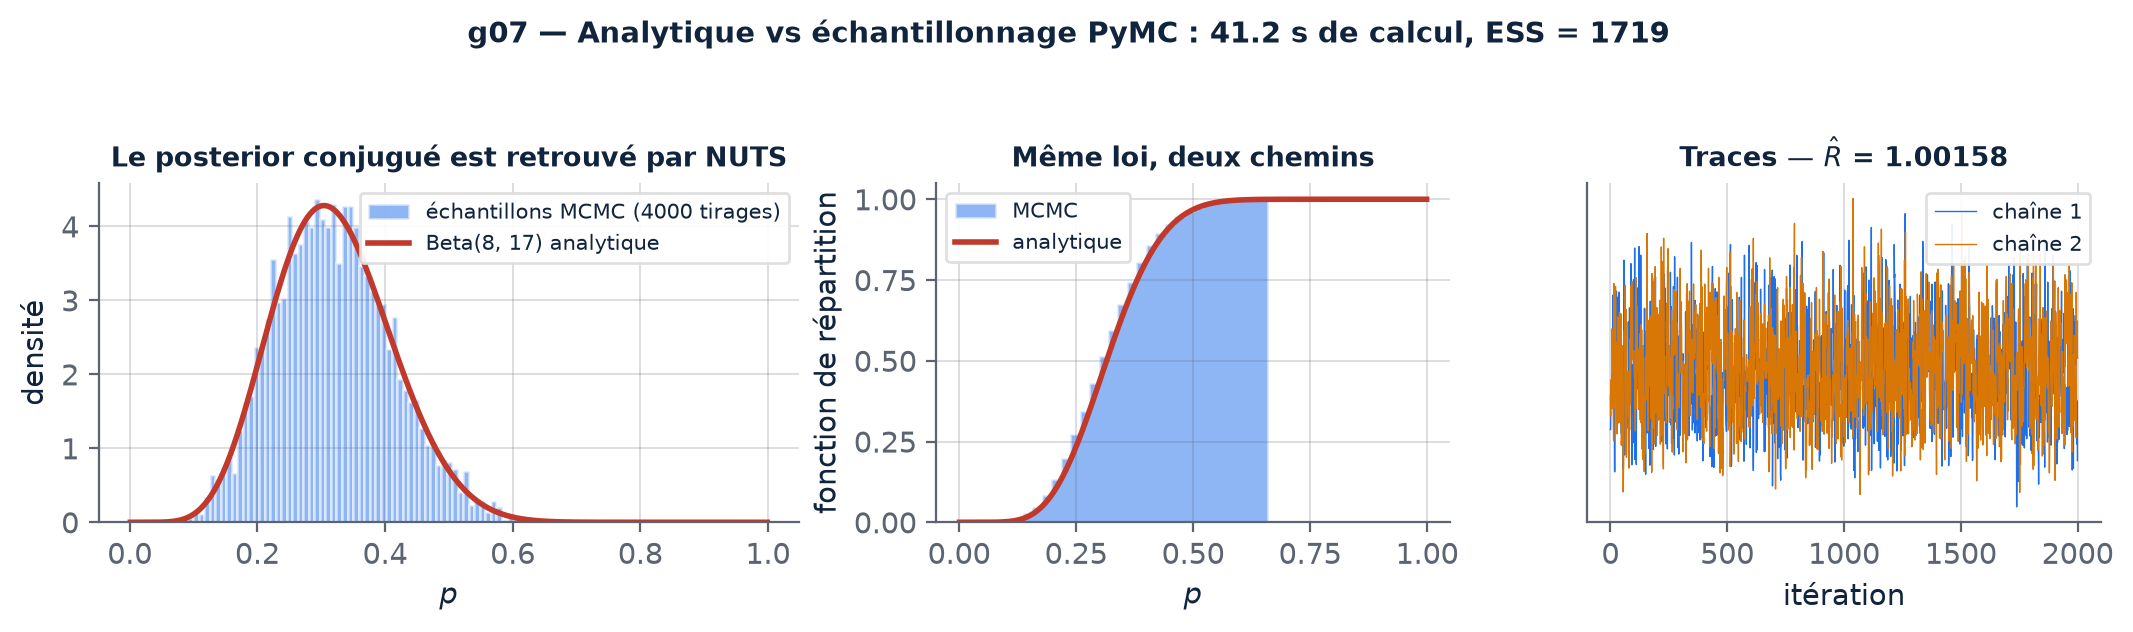
\includegraphics[width=.88\textwidth]{g07_analytique_vs_pymc.png}
\end{center}
\vspace{-1mm}
\begin{columns}[t]
\begin{column}{0.52\textwidth}
\begin{solbox}[Comparaison numérique]
\begin{tabular}{@{}lcc@{}}
\toprule
& \textbf{Exact} & \textbf{MCMC} \\
\midrule
loi du posterior & Beta$(8,17)$ & échantillons \\
moyenne & $0{,}3200$ & $0{,}3196$ \\
IC 95 \% bas & $0{,}1563$ & $0{,}1536$ \\
IC 95 \% haut & $0{,}5109$ & $0{,}5138$ \\
\bottomrule
\end{tabular}
\end{solbox}
\end{column}
\begin{column}{0.45\textwidth}
\begin{kbox}[La règle professionnelle]
On \textbf{valide toujours} un échantillonneur sur un cas conjugué avant de lui
confier un modèle sans forme close : ici $41{,}2$~s de calcul pour un résultat
déjà connu exactement. Les sections 2.2 à 2.4 n'utilisent que des cas où la
vérité est calculable.
\end{kbox}
\end{column}
\end{columns}
\end{frame}

% ---------------------------------------------------------------- 14
\begin{frame}{Lire un prior comme un échantillon virtuel}
\begin{ebox}[L'équation des débats sur les priors]
Pour le modèle Beta-Binomial, la moyenne a posteriori est une \textbf{moyenne pondérée}
entre le prior et les données :
\[
\underbrace{\hat p_{\post}}_{\text{posterior}}=
\underbrace{w}_{\text{poids du prior}} \cdot \underbrace{\frac{a}{a+b}}_{\text{moyenne du prior}}
\;+\;(1-w)\cdot \underbrace{\frac{k}{n}}_{\text{données}},
\qquad w = \frac{a+b}{a+b+n}
\]
\end{ebox}
\vspace{1mm}
\centering
\begin{tabular}{@{}p{1.8cm}p{0.9cm}p{1.3cm}p{1.8cm}p{2.3cm}p{3.9cm}@{}}
\toprule
\textbf{A priori} & $a+b$ & $w$ & \textbf{moy. post.} & \textbf{IC 95 \%} & \textbf{verdict} \\
\midrule
Beta$(1,1)$ & 2 & 0,080 & 0,3200 & $[0{,}156;0{,}511]$ & les données décident \\
Beta$(2,2)$ & 4 & 0,148 & 0,3333 & $[0{,}172;0{,}518]$ & presque neutre \\
Beta$(5,3)$ & 8 & 0,258 & 0,3871 & $[0{,}227;0{,}561]$ & avis marqué \\
Beta$(1{,}3;50)$ & 51,3 & \textbf{0,690} & 0,1117 & $[0{,}051;0{,}192]$ & \textbf{le prior domine} \\
\bottomrule
\end{tabular}
\vspace{1.5mm}
\begin{wbox}[Le piège des pseudo-observations]
Un $\mathrm{Beta}(50,50)$ encode \textbf{98} observations virtuelles et un
$w = 0{,}813$ face à 23 vols réels : convertir tout prior en \emph{taille
d'échantillon équivalente} avant de le dire neutre.
\end{wbox}
\end{frame}

% ---------------------------------------------------------------- 15
\begin{frame}{Quiz 1 — conjugaison en quatre questions}
\begin{qbox}[Question 3 -- Mise à jour]
\textbf{1.} On suppose $y_1,\dots,y_n \sim \mathrm{Poisson}(\lambda)$ et
$\lambda \sim \mathrm{Gamma}(2, 1)$. Après $n = 12$ et $\sum y_i = 48$,
quels sont les paramètres du posterior ? \\[1mm]
\textbf{2.} Même modèle, mais $\sum y_i = 48$ et $n = 240$ : quel prior pèse
le plus, et pourquoi ? \\[1mm]
\textbf{3.} Pour une proportion $p$, quels hyperparamètres encode un avis « autour
de 0,3, plutôt précis » ? Et un avis « entre 0,1 et 0,5 sans plus » ? \\[1mm]
\textbf{4.} Un collègue écrit : « prior Beta$(0{,}5;0{,}5)$ = pas d'information ».
A-t-il raison ?
\vspace{2mm}

\textcolor{byBlue}{\textbf{Réponses :}}
\textbf{1.} $\mathrm{Gamma}(2+48,\,1+12) = \mathrm{Gamma}(50,13)$, moyenne
$3{,}846$. \quad
\textbf{2.} Poids $w = 3/(3+240) = 0{,}012$ : le prior est écrasé (vs $3/15 = 0{,}20$). \quad
\textbf{3.} Beta$(15,35)$ (moy. 0,3000, é.-t. 0,0642) contre Beta$(2,4)$ (moy. 0,3333, é.-t. 0,1782). \quad
\textbf{4.} Non : c'est le prior de \textbf{Jeffreys}, le moins informatif qui garde
une invariance ; mais il favorise 0 et 1, ce qui est une information (section 2.2).
\end{qbox}
\end{frame}

% ---------------------------------------------------------------- 16
\begin{frame}{Activité guidée — dériver un posterior à la main (8 min)}
% [rogna]
\small
\begin{abox}[Consigne, par binôme]
On observe une pièce lancée $n = 10$ fois, donnant $k = 3$ faces.
Prior : $\theta \sim \mathrm{Beta}(2,2)$.
\begin{enumerate}
  \item Écrire $p(\theta)$ et le noyau de la vraisemblance.
  \item Multiplier, puis \textbf{identifier} les paramètres du posterior.
  \item Calculer la moyenne a posteriori à la main, puis vérifier avec le script.
  \item Répondre : $P(\theta > 0{,}5 \given y)$ est-elle supérieure à 0,2 ?
\end{enumerate}
\end{abox}
\vspace{1mm}
\begin{columns}[t]
\begin{column}{0.55\textwidth}
\begin{solbox}[Correction détaillée]
\[
p(\theta) \propto \theta^{1}(1-\theta)^{1}, \qquad
p(y \given \theta) \propto \theta^{3}(1-\theta)^{7}
\]
\[
p(\theta \given y) \propto \theta^{4}(1-\theta)^{8}
= \mathrm{Beta}(5, 9)
\]
Moyenne : $\frac{5}{5+9} = \mathbf{0{,}3571}$.
Poids du prior : $w = \frac{2+2}{4+10} = 0{,}2857$.
Vérification directe par la formule pondérée :
$0{,}2857 \times 0{,}5 + 0{,}7143 \times 0{,}3 = 0{,}3571$.
\end{solbox}
\end{column}
\begin{column}{0.42\textwidth}
\begin{ebox}[Contrôle par la loi exacte]
$\mathrm{Beta}(5,9)$ : $P(\theta > 0{,}5) = 0{,}1334$ (calcul SciPy).
La réponse au point 4 est donc \textbf{non} : malgré $k/n = 0{,}3$ et un prior
centré sur 0,5, la probabilité que la pièce soit biaisée vers face reste faible.
La conclusion s'énonce toujours avec la question posée : « biaisée vers
\emph{face} », pas « truquée ».
\end{ebox}
\end{column}
\end{columns}
\end{frame}

% ---------------------------------------------------------------- 17
\begin{frame}{Synthèse 2.1 — ce qu'il faut avoir retenu}
% [rogna]
\footnotesize
\begin{kbox}[Les cinq acquis de la conjugaison]
\begin{enumerate}
  \item Le posterior s'obtient en \textbf{reconnaissant un noyau} : la constante de
        normalisation ne se calcule jamais.
  \item Les quatre couples (Beta-Binomial, Gamma-Poisson, Normal-Normal,
        Dirichlet-Multinomial) couvrent l'essentiel des cas d'usage.
  \item Les hyperparamètres se lisent comme des \textbf{comptes de données
        virtuelles} : $w = \frac{a+b}{a+b+n}$ mesure la force du prior.
  \item La conjugaison est \textbf{exacte et instantanée} : elle sert de banc
        d'essai pour les échantillonneurs du chapitre 5.
  \item Un prior informatif peut renverser une conclusion : sur Challenger, la
        moyenne passe de $0{,}320$ à $0{,}112$.
\end{enumerate}
\end{kbox}
\vspace{-2mm}
\begin{columns}[t]
\begin{column}{0.54\textwidth}
\begin{ebox}[Passerelle vers la section 2.2]
La conjugaison suppose la famille de priors choisie. La vraie question n'est donc
pas « comment calculer ? » mais « \textbf{quel prior écrire, et comment le
justifier} ? ». C'est l'objet de la section suivante.
\end{ebox}
\end{column}
\begin{column}{0.42\textwidth}
\begin{wbox}[Trois erreurs à ne plus commettre]
\warn{} confondre précision et faible influence : un prior très resserré est très
influent ; \;
\warn{} oublier que le posterior \emph{dépend} du prior ; \;
\warn{} conclure sans donner l'intervalle de crédibilité.
\end{wbox}
\end{column}
\end{columns}
\end{frame}
